\documentclass[11pt]{article}

% Packages
\usepackage[utf8]{inputenc}
\usepackage[T1]{fontenc}
\usepackage{amsmath}
\usepackage{amsthm}
\usepackage{amssymb}
\usepackage{graphicx}
\usepackage{caption}
\usepackage{hyperref}
\hypersetup{colorlinks=true, linkcolor=blue, citecolor=blue, urlcolor=blue}
\usepackage{url}
\usepackage[numbers]{natbib}
\usepackage{geometry}
\geometry{margin=1in}

% Custom commands
\renewcommand{\v}[1]{\boldsymbol{#1}}

% Theorem environments
\newtheorem{theorem}{Theorem}[section]
\newtheorem{property}{Property}[section]
\newtheorem{remark}{Remark}[section]

% Title and author information
\title{When Does Model Simplification Matter?\\Consequence Analysis for Weibull Series Systems}
\author{
  \Large{Alex Towell} \\
  Department of Computer Science \\
  Southern Illinois University Edwardsville \\
  \href{mailto:lex@metafunctor.com}{lex@metafunctor.com}
}
\date{}

\begin{document}

\maketitle

\begin{abstract}
When a reliability engineer simplifies a series system model by assuming all components share a common Weibull shape parameter, how much accuracy is lost---and can the data even tell the difference? We show that these two questions have a favorably aligned answer: the likelihood ratio test's power outpaces the reduced model's prediction bias. The common-shape model's MTTF bias remains below 1\% through shape CV $\approx 15\%$, and by the time it reaches 1.5\% (CV $\approx 20\%$) the LRT already rejects at nearly 80\%. This means the test lacks power only where the consequence of using the wrong model is negligible. An adaptive LRT-based procedure exploits this alignment, achieving RMSE within 2.5\% of the full model at $n \geq 500$ while selecting the simpler model over 90\% of the time when appropriate. All results are obtained under realistic conditions of right-censored and masked failure data.
\end{abstract}

\section{Introduction}

Consider a turbine engine whose operation depends on bearings, seals, and blades arranged in series---any component failure grounds the engine. Field maintenance logs record the failure time and a short list of suspect components (the candidate set), but exact root-cause analysis requires costly teardown. Warranty programs further right-censor units still in service. The engineer faces a fundamental modeling choice: a full model with separate Weibull shape and scale parameters for each of $m$ components ($2m$ parameters), or a reduced model that assumes a common shape parameter across all components ($m+1$ parameters).

The full model is more flexible but harder to estimate with limited masked data. The reduced model is more parsimonious and---uniquely among single-parameter reductions---renders the system lifetime itself Weibull \cite{barlow1975}, enabling closed-form reliability metrics. But is the simplification safe? The existing literature on this question focuses almost entirely on whether a likelihood ratio test can \emph{detect} the difference between models \cite{towell2023reliability}. This is the wrong question. The right question is: when the reduced model is wrong, does it produce predictions that are wrong enough to change an engineering decision?

\subsection{Related Work}

Maximum likelihood estimation from masked series system data has been developed through frequentist \cite{Usher-1988, Lin-1993, Joh-1989} approaches. Guo et al.\ \cite{Huairu-2013} provide the baseline system configuration used in our simulations, and Towell \cite{towell2023reliability} developed the likelihood model incorporating both right-censoring and candidate sets that we use throughout.

The Weibull closure property under common shape is classical \cite{barlow1975}. Craiu and Lee \cite{Craiu-2005} addressed model selection for competing-risks models with masking, but not in the Weibull series system context. The model selection question---common shape versus heterogeneous shapes---has not, to our knowledge, been studied systematically for masked data, nor has the consequence of misspecification been quantified. We employ the likelihood ratio test \cite{wilks1938} and compare with AIC \cite{akaike1974} and BIC \cite{schwarz1978}.

\subsection{Contributions}

\begin{enumerate}
\item \textbf{Bias-detectability alignment}: MTTF bias remains below 1\% through CV $\approx 15\%$; by CV $\approx 20\%$ (bias 1.5\%), the LRT already rejects at nearly 80\%. Surprisingly, the full model has lower MTTF variance than the reduced model at moderate sample sizes ($n \leq 1000$), even at CV $= 0$, because the nonlinear MTTF functional amplifies the constrained estimator's variance more than the unconstrained estimator's.

\item \textbf{Adaptive model selection}: An LRT-based procedure exploits this alignment, achieving RMSE within 2.5\% of the always-full strategy at $n \geq 500$ while selecting the simpler model $> 90\%$ of the time when the data support it.
\end{enumerate}

%% =========================================================================
\section{Model Framework}
\label{sec:framework}

\subsection{Series System with Weibull Components}

Consider a series system of $m$ independent components, where the system fails when any component fails. Each component lifetime $T_j$ follows a two-parameter Weibull distribution with shape $k_j > 0$ and scale $\lambda_j > 0$:
\begin{equation}
f_j(t; k_j, \lambda_j) = \frac{k_j}{\lambda_j}\left(\frac{t}{\lambda_j}\right)^{k_j-1} \exp\left\{-\left(\frac{t}{\lambda_j}\right)^{k_j}\right\}, \quad t > 0.
\end{equation}
The system lifetime $T = \min\{T_1, \ldots, T_m\}$ has reliability function
\begin{equation}
\label{eq:sys_reliability}
R(t;\v\theta) = \exp\biggl\{-\sum_{j=1}^{m}\biggl(\frac{t}{\lambda_j}\biggr)^{k_j}\biggr\},
\end{equation}
with hazard $h(t;\v\theta) = \sum_j (k_j/\lambda_j)(t/\lambda_j)^{k_j-1}$ and density $f = h \cdot R$,
where $\v\theta = (k_1, \lambda_1, \ldots, k_m, \lambda_m)$ is the full parameter vector and $\text{MTTF}_j = \lambda_j \Gamma(1 + 1/k_j)$.

\subsection{Masked and Censored Data}

We observe $n$ independent system lifetimes under two forms of incomplete information:
\begin{itemize}
\item \textbf{Right-censoring}: Some systems are still operating at the end of the observation period. For system $i$, $\delta_i = 1$ indicates failure and $\delta_i = 0$ indicates censoring.
\item \textbf{Masking}: For failed systems, only a candidate set $C_i \subseteq \{1, \ldots, m\}$ of possible failure causes is observed, not the true failed component $K_i$. The candidate set always contains the true cause ($K_i \in C_i$), and the masking mechanism is non-informative about $\v\theta$ \cite{towell2023reliability}.
\end{itemize}

The log-likelihood for the complete sample is
\begin{equation}
\label{eq:loglik}
\ell(\v\theta) = \sum_{i=1}^{n} \left[ (1-\delta_i) \log R(t_i; \v\theta) + \delta_i \log \left( \sum_{j \in C_i} \frac{h_j(t_i)}{h(t_i; \v\theta)} \cdot f(t_i; \v\theta) \right) \right],
\end{equation}
which is maximized numerically using the L-BFGS-B algorithm \cite{byrd1995} with analytical gradients. For details, see \cite{towell2023reliability}.

\subsection{The Common-Shape Model}

The \emph{common-shape model} (reduced model) constrains all components to share a single shape parameter $k$, with parameter vector $\v\theta_R = (k, \lambda_1, \ldots, \lambda_m)$. This reduces the parameter count from $2m$ to $m+1$.

\begin{property}[Weibull Closure {\cite{barlow1975}}]
\label{prop:weibull-closure}
Let $T_1, \ldots, T_m$ be independent with $T_j \sim \text{Weibull}(k, \lambda_j)$. Then $T = \min\{T_1, \ldots, T_m\} \sim \text{Weibull}(k, \lambda_s)$ where $\lambda_s = (\sum_{j=1}^{m} \lambda_j^{-k})^{-1/k}$.
\end{property}

The common-shape constraint is the \emph{only} single-parameter restriction that yields a Weibull system lifetime, making it the natural parsimony boundary. The key practical question is not whether the property holds exactly, but whether predictions from the common-shape model are adequate when shapes are \emph{approximately} equal.

In well-designed systems, components age similarly ($k_j \approx k$) but differ in durability ($\lambda_j$), making the common-shape model a physically motivated reduction.

\subsection{Baseline System and Simulation Design}
\label{sec:baseline}

We measure departure from shape homogeneity by the coefficient of variation $\text{CV}_k = \text{sd}(k_1,\ldots,k_m)/\text{mean}(k_1,\ldots,k_m)$. Throughout this paper, we use a 5-component baseline system from \cite{Huairu-2013} with $\text{CV}_k \approx 4\%$:

\begin{table}[htbp]
\centering
\caption{Baseline 5-Component Series System}
\label{tab:series-sys}
\begin{tabular}{cccc}
\hline
Component $j$ & Shape $k_j$ & Scale $\lambda_j$ & MTTF$_j$ \\
\hline
1 & 1.2576 & 994.37 & $\approx 913$ \\
2 & 1.1635 & 908.95 & $\approx 859$ \\
3 & 1.1308 & 840.11 & $\approx 799$ \\
4 & 1.1802 & 940.13 & $\approx 886$ \\
5 & 1.2034 & 923.16 & $\approx 866$ \\
\hline
\end{tabular}
\end{table}

All simulations use masking probability $p = 0.215$ and censoring quantile $q = 0.825$. To vary shape heterogeneity, we generate $m$ shapes uniformly spaced about a mean of 1.18 with a specified target CV. Because the shapes are discrete, the realized CV differs slightly from the target (e.g., target CV $= 10\%$ yields actual CV $\approx 13.7\%$). All tables and figures report the actual CV; approximate values are used in prose for readability. All simulations use the \texttt{wei.series.md.c1.c2.c3} R package \cite{towell2023weibull} with L-BFGS-B optimization \cite{byrd1995} and analytical gradients. A sensitivity analysis in \cite{towell2023reliability} shows that MLE precision depends strongly on component failure probability and that shape parameters are inherently harder to estimate than scale parameters---even without masking or censoring---both observations motivating the common-shape reduction studied here.

%% =========================================================================
\section{Consequence Analysis: Does Model Misspecification Matter?}
\label{sec:consequences}

The central question is not whether the common-shape model is statistically distinguishable from the full model, but whether it produces predictions that are wrong enough to affect engineering decisions. We quantify this by fitting the reduced model to data generated from heterogeneous-shape systems and measuring the resulting prediction errors.

\subsection{Simulation Design}

For each simulation replication, we compute the system MTTF $= \int_0^\infty R(t; \v\theta)\, dt$ under both the fitted full and reduced models, and measure the relative bias $(\widehat{\text{MTTF}} - \text{MTTF}_{\text{true}}) / \text{MTTF}_{\text{true}}$. We varied shape CV across 9 levels (0--30\%) and sample sizes $n \in \{100, 500, 1000, 5000\}$, with 500 replications per condition. Non-convergent fits (typically $< 3\%$; up to 10\% at extreme CV) are excluded.

\subsection{Results}

Table~\ref{tab:consequence} summarizes the reduced model's MTTF bias across shape CV and sample size.

\begin{table}[htbp]
\centering
\caption{Reduced Model MTTF Bias (\%) and RMSE (in time units) by Actual Shape CV and Sample Size}
\label{tab:consequence}
\small
\begin{tabular}{ccccccccc}
\hline
& \multicolumn{2}{c}{$n=100$} & \multicolumn{2}{c}{$n=500$} & \multicolumn{2}{c}{$n=1000$} & \multicolumn{2}{c}{$n=5000$} \\
CV (\%) & Bias & RMSE & Bias & RMSE & Bias & RMSE & Bias & RMSE \\
\hline
0.0 & $+$0.4 & 20.4 & $-$0.1 & 9.6 & $+$0.0 & 6.8 & $-$0.0 & 2.9 \\
2.7 & $+$0.3 & 21.0 & $-$0.1 & 10.0 & $-$0.1 & 6.9 & $+$0.0 & 2.9 \\
5.5 & $+$0.8 & 21.2 & $+$0.2 & 9.3 & $+$0.1 & 6.6 & $+$0.1 & 3.1 \\
8.2 & $+$0.7 & 20.5 & $+$0.5 & 9.5 & $+$0.1 & 6.6 & $+$0.2 & 3.0 \\
11.0 & $+$1.1 & 21.5 & $+$0.6 & 9.8 & $+$0.2 & 6.7 & $+$0.2 & 3.0 \\
13.7 & $+$0.8 & 21.8 & $+$0.9 & 10.1 & $+$0.5 & 7.0 & $+$0.6 & 3.3 \\
20.5 & $+$1.7 & 23.9 & $+$1.5 & 10.5 & $+$1.3 & 7.7 & $+$1.3 & 4.2 \\
27.4 & $+$3.2 & 23.9 & $+$2.9 & 12.5 & $+$2.5 & 9.2 & $+$2.6 & 6.4 \\
41.1 & $+$10.5 & 37.4 & $+$10.1 & 23.1 & $+$9.8 & 20.8 & $+$9.3 & 18.2 \\
\hline
\end{tabular}
\end{table}

Three patterns emerge. First, the reduced model's MTTF bias is remarkably small: below 1\% through shape CV $\approx 14\%$ at $n \geq 500$, and the 1\% threshold is not crossed until CV $\approx 20\%$ (bias $= 1.5\%$). Only at CV $> 27\%$ does the bias exceed 2.5\%. Second, the bias is almost entirely positive---the reduced model systematically overestimates MTTF because the common-shape fit overestimates the weaker components. Third, the bias is largely independent of sample size: a 50-fold increase from $n = 100$ to $n = 5000$ changes the bias at CV $\approx 27\%$ from $+3.2\%$ to $+2.6\%$, confirming that this is a specification bias, not a finite-sample artifact.

\subsection{Discussion}

A surprising finding is that the full model has lower MSE than the reduced model at moderate sample sizes ($n \leq 1000$)---even when the reduced model is correctly specified (CV $= 0$). A bias-variance decomposition reveals the mechanism: the constraint $k_1 = \cdots = k_m$ forces all shape estimation error into a single degree of freedom, which propagates through the nonlinear MTTF integral with greater amplification than the distributed errors of the unconstrained estimator \cite{White-1982}. The traditional argument that parsimony reduces variance holds for the shape parameters themselves, but not for the system MTTF. The case for the common-shape model rests instead on interpretability, the Weibull closure property, and the empirical observation that its predictions are accurate enough for engineering use when shape heterogeneity is modest.

Figure~\ref{fig:alignment} reveals the quantitative alignment between detectability and consequence. The LRT's power curve rises faster than the bias curve: by the time the MTTF bias reaches engineering-significant levels, the LRT already rejects reliably. This rate asymmetry is what makes the adaptive procedure in Section~\ref{sec:adaptive} effective.

\begin{figure}[htbp]
\centering
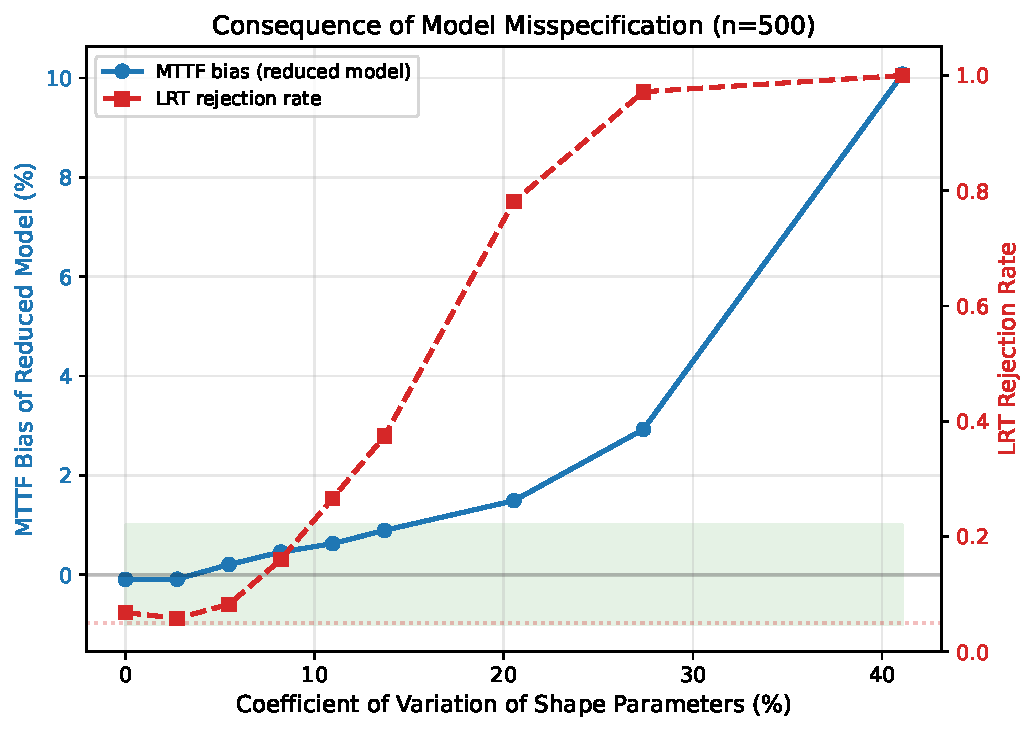
\includegraphics[width=0.85\textwidth]{image/consequence_focused.pdf}
\caption{The alignment between prediction consequence and statistical detectability at $n = 500$. Left axis (blue): MTTF bias of the reduced model. Right axis (red): LRT rejection rate. The green band marks the $\pm 1\%$ engineering-acceptable bias zone. Detection power outpaces prediction bias: the test lacks power precisely where bias is negligible, and reaches high power before bias becomes engineering-significant.}
\label{fig:alignment}
\end{figure}

%% =========================================================================
\section{Likelihood Ratio Testing}
\label{sec:lrt}

We employ the likelihood ratio test (LRT) with statistic
\begin{equation}
\Lambda = -2 (\ell(\hat{\v\theta}_R) - \ell(\hat{\v\theta}_F)),
\end{equation}
which is asymptotically $\chi^2_{m-1}$ under the null hypothesis $H_0: k_1 = \cdots = k_m$ \cite{wilks1938}.

\subsection{Type I Error and Power}

Under perfect homogeneity ($\text{CV}_k = 0$), the LRT rejection rate ranges from 4.6\% to 6.8\% across all sample sizes tested ($n = 100$ to $10{,}000$), confirming well-calibrated Type~I error at the nominal $\alpha = 0.05$.

Table~\ref{tab:power-by-cv} presents the LRT rejection rate (power) as a function of shape CV for different sample sizes.

\begin{table}[htbp]
\centering
\caption{LRT Rejection Rate by Divergence Level and Sample Size}
\label{tab:power-by-cv}
\small
\begin{tabular}{cccccc}
\hline
CV (\%) & $n = 100$ & $n = 500$ & $n = 1000$ & $n = 5000$ & $n = 10000$ \\
\hline
0.0 & 0.054 & 0.056 & 0.046 & 0.068 & 0.046 \\
2.7 & 0.048 & 0.062 & 0.052 & 0.186 & 0.268 \\
5.5 & 0.075 & 0.072 & 0.130 & 0.541 & 0.887 \\
8.2 & 0.074 & 0.126 & 0.266 & 0.936 & 0.996 \\
11.0 & 0.088 & 0.252 & 0.494 & 0.996 & 1.000 \\
\hline
\end{tabular}
\end{table}

The key observation: at CV $\leq 5\%$, the LRT has almost no power at practical sample sizes ($n \leq 1000$). Even at $n = 10{,}000$, the rejection rate at CV $= 2.7\%$ is only 27\%. Combined with the consequence analysis showing that prediction bias is negligible in this regime, the case for the common-shape model is strong.

Appendix~\ref{app:data-quality} examines how masking probability, censoring level, and system complexity affect LRT power. In brief: masking has the largest impact ($6\times$ power reduction from $p = 0.05$ to $p = 0.70$), followed by censoring ($2.5\times$), but neither factor inflates the Type~I error rate. Appendix~\ref{app:aic-bic} compares the LRT with AIC and BIC; the LRT is well-calibrated (4.6--6.8\% Type~I error at $\alpha = 0.05$), while AIC is liberal (${\approx}\,2\times$) and BIC over-conservative (${\leq}\,0.2\%$).

%% =========================================================================
\section{Adaptive Model Selection}
\label{sec:adaptive}

\subsection{Procedure}

Given data from an unknown system, we evaluate a natural LRT-based adaptive procedure: fit both models, compute $\Lambda = -2(\ell(\hat{\v\theta}_R) - \ell(\hat{\v\theta}_F))$, and use the reduced model if $\Lambda < \chi^2_{m-1, 1-\alpha}$. Under the null, this selects the reduced model with probability $1 - \alpha$.

\subsection{Simulation Design}

We compare three strategies:
\begin{enumerate}
\item \textbf{Always-full}: use full model estimates regardless
\item \textbf{Always-reduced}: use reduced model estimates regardless
\item \textbf{Adaptive (LRT)}: select model via the LRT at $\alpha = 0.05$
\end{enumerate}

We evaluate on MTTF estimation accuracy (MSE, bias) across shape CV from 0 to 20\% and sample sizes $n \in \{100, 500, 1000\}$, with 500 replications per condition. Non-convergent fits are excluded (typically $< 2\%$ of replications).

\subsection{Results}

Table~\ref{tab:adaptive} presents the RMSE of each strategy as a percentage of the true system MTTF, along with the fraction of replications where the LRT-based adaptive procedure selects the reduced model. Figure~\ref{fig:adaptive} provides the corresponding visualization.

\begin{table}[htbp]
\centering
\caption{Adaptive Model Selection: RMSE (\% of True MTTF) and Selection Rate}
\label{tab:adaptive}
\small
\begin{tabular}{cccccc}
\hline
CV (\%) & $n$ & Full & Reduced & Adaptive & Sel.~Red. (\%) \\
\hline
0.0 & 100 & 9.3 & 10.1 & 10.0 & 93 \\
    & 500 & 4.6 & 4.7 & 4.7 & 95 \\
    & 1000 & 3.0 & 3.0 & 3.0 & 94 \\
\hline
5.5 & 100 & 9.3 & 10.1 & 10.1 & 95 \\
    & 500 & 4.1 & 4.2 & 4.2 & 92 \\
    & 1000 & 3.0 & 3.0 & 3.1 & 89 \\
\hline
13.7 & 100 & 9.5 & 10.4 & 10.3 & 89 \\
     & 500 & 4.3 & 4.5 & 4.4 & 60 \\
     & 1000 & 3.0 & 3.2 & 3.0 & 30 \\
\hline
20.5 & 100 & 9.5 & 10.7 & 10.4 & 83 \\
     & 500 & 4.4 & 4.9 & 4.5 & 21 \\
     & 1000 & 3.2 & 3.6 & 3.2 & 1 \\
\hline
27.4 & 100 & 9.9 & 12.8 & 11.6 & 65 \\
     & 500 & 4.6 & 5.6 & 4.7 & 1 \\
     & 1000 & 3.3 & 4.4 & 3.3 & 0 \\
\hline
\end{tabular}
\end{table}

\begin{figure}[htbp]
\centering
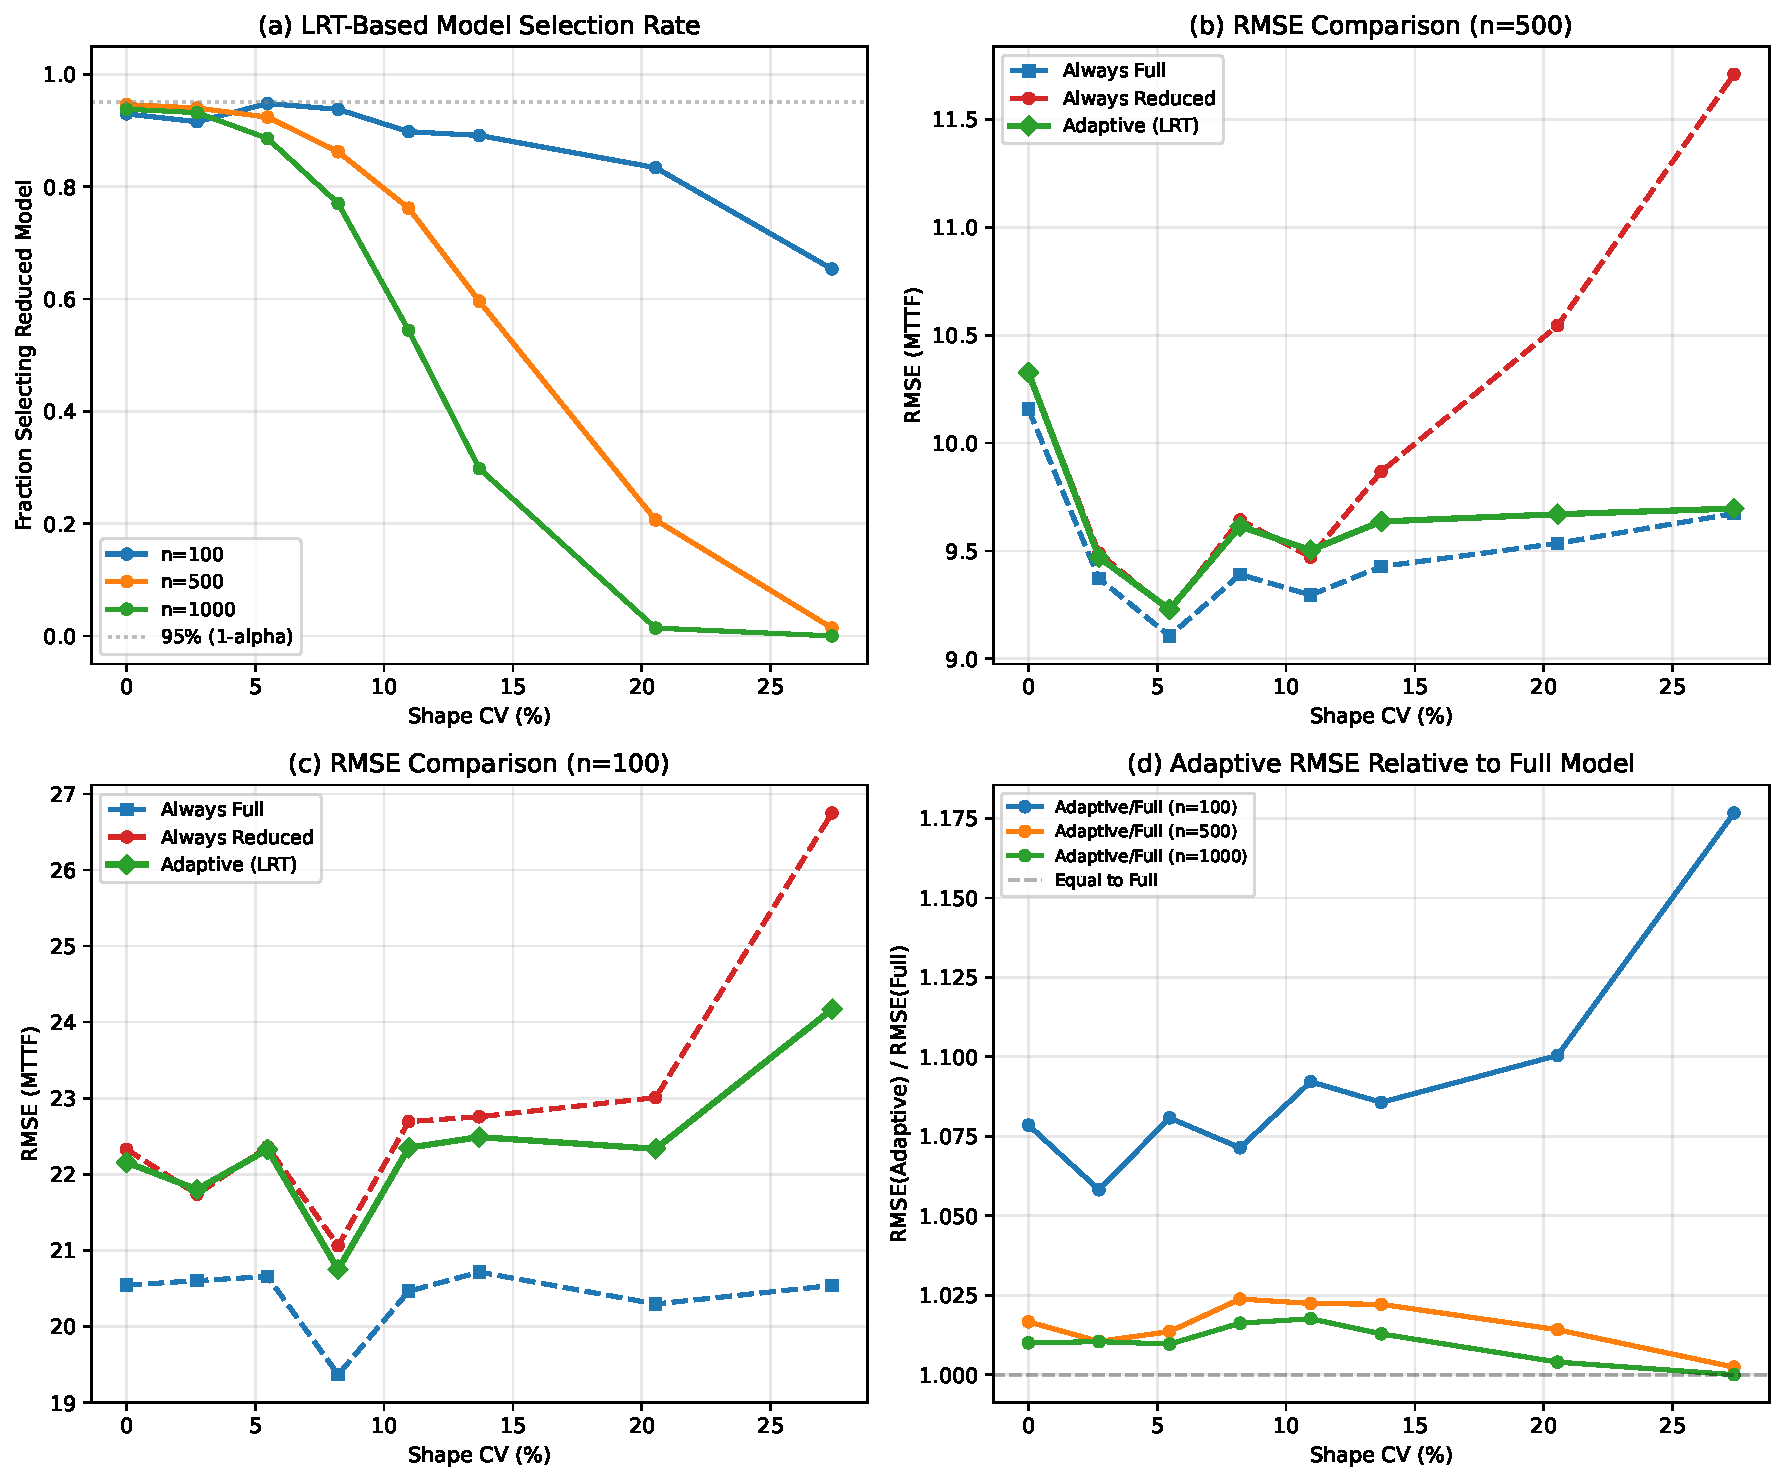
\includegraphics[width=0.85\textwidth]{image/adaptive_selection.pdf}
\caption{Adaptive model selection. (a)~Selection rate: the LRT correctly selects the reduced model near 95\% at CV~$= 0$ and transitions smoothly to the full model as CV increases, with the transition point shifting left with sample size. (b)--(c)~RMSE comparison at $n = 500$ and $n = 100$: the adaptive procedure (green) tracks the better of the two static strategies across all CVs. (d)~Relative RMSE: the adaptive procedure's overhead ranges from 8--18\% at $n = 100$ and is under 2.5\% at $n = 500$.}
\label{fig:adaptive}
\end{figure}

The adaptive procedure selects the reduced model $> 90\%$ of the time at low CV and transitions smoothly to the full model as heterogeneity increases. The RMSE overhead relative to always-full is at most 2.4\% at $n = 500$. At $n = 100$ the overhead is larger (8--18\%) because the LRT lacks power, but the consequence analysis (Table~\ref{tab:consequence}) shows the reduced model's bias is still moderate at those CVs.

\subsection{Discussion}

The adaptive procedure succeeds because of the bias-detectability alignment (Figure~\ref{fig:alignment}): the LRT has low power precisely where the consequence of misspecification is small, and high power where the consequence is large. The ``incorrect'' selections at moderate CV carry negligible penalty because the reduced model's bias is still below 1\% at those CVs. Since both fits are already required to compute $\Lambda$, the procedure adds no cost.

%% =========================================================================
\section{Conclusion}
\label{sec:conclusion}

This paper addressed a fundamental question in reliability engineering: when can practitioners safely simplify a Weibull series system model by assuming common component shapes? The answer is structured around a quantitative alignment between prediction consequence and statistical detectability.

\paragraph{The LRT's power outpaces the reduced model's prediction bias.}
The common-shape model's MTTF bias remains below 1\% through CV $\approx 15\%$, and by the time it reaches 1.5\% (CV $\approx 20\%$) the LRT already rejects at nearly 80\%. The test lacks power precisely where misspecification is harmless, and has high power precisely where the bias warrants switching to the full model. An adaptive LRT-based procedure exploits this alignment, achieving RMSE within 2.5\% of the always-full strategy at $n \geq 500$ while selecting the simpler model over 90\% of the time when the data support it.

\paragraph{The traditional argument for the reduced model does not hold.}
At moderate sample sizes ($n \leq 1000$), the full model has lower MTTF variance even at CV $= 0$; the case for the common-shape model rests on interpretability, Weibull closure, and engineering-adequate predictions across a broad range of shape heterogeneity.

\paragraph{Limitations.}
Our simulations use uniformly spaced shapes about a common mean. Real systems may exhibit asymmetric or clustered heterogeneity patterns. The single baseline system (5 components, moderate masking and censoring) may not capture all configurations of practical interest.

\paragraph{Future directions.}
Extending to non-Weibull distributions (where analogous closure properties may or may not hold) and to parallel or $k$-out-of-$n$ configurations would broaden applicability.

\appendix

\section{Data Quality Effects on LRT Power}
\label{app:data-quality}

We varied masking probability ($p$), censoring quantile ($q$), and number of components ($m$) for the baseline system (CV $\approx 4\%$). Table~\ref{tab:data-quality} summarizes the effects at $n = 5000$. Masking has the largest impact ($6\times$ power reduction from $p = 0.05$ to $p = 0.70$), followed by censoring ($2.5\times$). Larger systems have lower power due to higher critical values and failure information distributed across more parameters. Importantly, no factor inflates the Type~I error rate---the test remains well-calibrated throughout.

\begin{table}[htbp]
\centering
\caption{Effect of Data Quality Factors on LRT Power ($n = 5000$, Baseline System)}
\label{tab:data-quality}
\small
\begin{tabular}{llcc}
\hline
Factor & Range & Power Range & Effect \\
\hline
Masking $p$ & 0.05--0.70 & 48\% $\to$ 8\% & $6\times$ reduction \\
Censoring $q$ & 0.50--1.00 & 17\% $\to$ 43\% & $2.5\times$ increase \\
Components $m$ & 2--8 & 77\% $\to$ 16\% & $5\times$ reduction \\
\hline
\end{tabular}
\end{table}

\section{Comparison with Information Criteria}
\label{app:aic-bic}

Figure~\ref{fig:lrt-vs-aic-bic} compares the LRT with AIC \cite{akaike1974} and BIC \cite{schwarz1978}. Under perfect homogeneity (CV $= 0$), the LRT is well-calibrated (4.6--6.8\%), AIC is liberal (8.2--12.4\%, with false positive rate increasing with $n$ because its fixed penalty does not scale), and BIC is over-conservative (${\leq}\,0.2\%$), making it unsuitable for detecting the subtle heterogeneity characteristic of well-designed systems.

\begin{figure}[htbp]
\centering
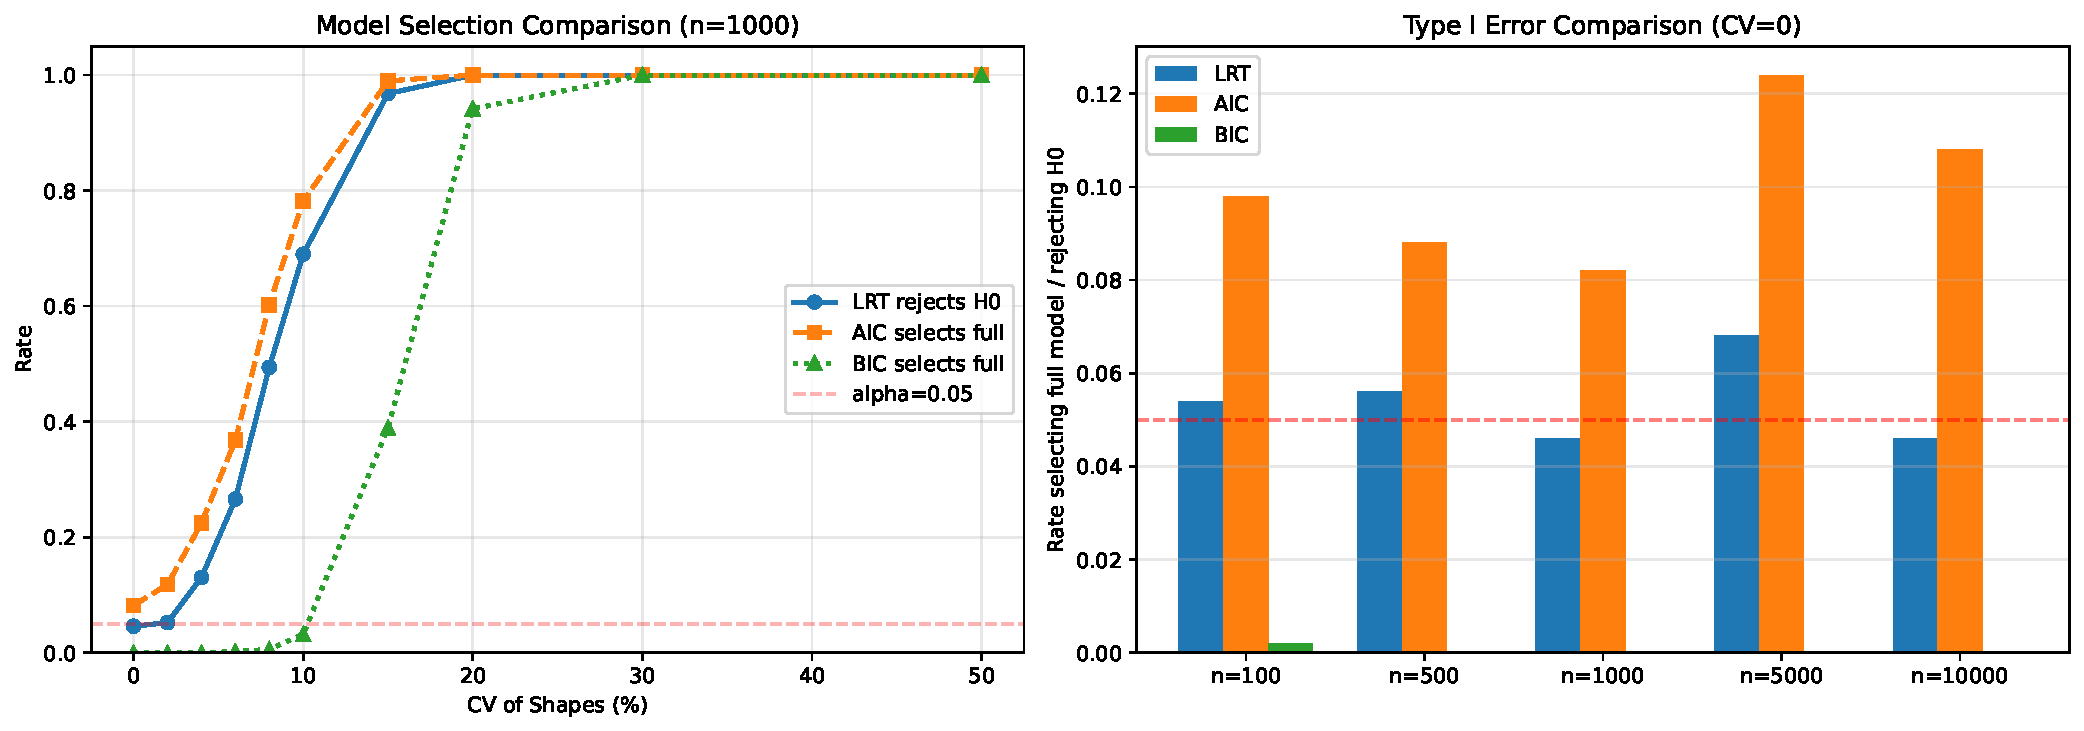
\includegraphics[width=0.85\textwidth]{image/lrt_vs_aic_bic_divergence.pdf}
\caption{Model selection rates for LRT ($\alpha = 0.05$), AIC, and BIC vs shape CV.}
\label{fig:lrt-vs-aic-bic}
\end{figure}

\bibliographystyle{IEEEtranN}
\bibliography{refs}

\end{document}
